\chapter{DLC}

\section{růst DLC}

\subsection{Procesy v plazmatu}
Mezi klíčové parametry depozice patří vhodné zvolení depozičního plynu. Běžně používané plyny pro depozice a-C:H vrstev jsou jednoduché uhlovodíkové sloučeniny jako alkany (např. methan, ethan, propan, butan ...), alkeny (např. ethen), alkyny (např. acetylen), aromatické uhlovodíky (benzen) a další. Důležité parametry použitého plynu jsou ionizační energie, molekulární hmotnost a poměr vodíku k uhlíku. Pro nižší ionizační energie se rychlost depozice zvětšuje přibližně exponenciálně \cite{"robertson[4]"}. Celková molekulová hmotnost je důležitá proto, že vlastnosti výsledné vrstvy závisí hlavně na energii dopadu v přepočtu na jeden atom a tak například benzenový iont C$_6$H$_6^+$ potřebuje přibližně šestkrát vyšší napětí pro urychlení než iont methanu. Z poměru uhlíku a vodíku 

Pro depozici tvrdých ochranných vrstev se nejčastěji používá acetylen (C$_2$H$_2$), protože má po metanu nejnižší molekulovou hmotnost, nízkou ionizační energii FIXME, nízký obsah vodíku a sníženou míru plazmové polymerizace. Nevýhoda je, že není dostupný v čisté formě a obsahuje nějaké nečistoty jako například dusík \cite{Conway2000}. Z toho důvodu je pro depozici vrstev určených k optické charakterizaci nevhodný. Pro výrobu vrstev byl proto zvolen metan, který má sice vysokou ionizační potenciál (cca 12,4\,V), ale neobsahuje příměsi a kvůli jeho nízké hmotnosti není potřeba příliš velké předpětí při depozici.





sp2 sp3, vodík...

relaxovaný stav

vlastnosti

atd, atd...

\section{Kapacitně vázaný vysokofrekvenční výboj}

\begin{figure}[htbp]
  \centering
  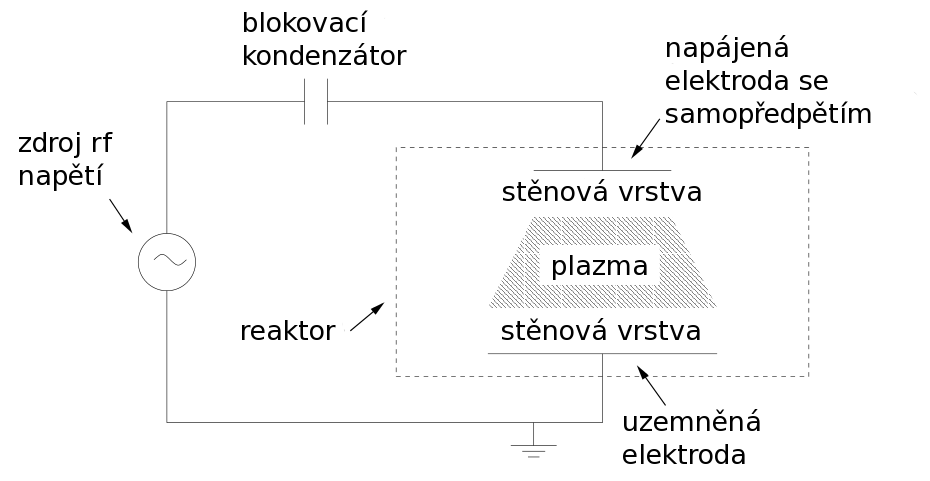
\includegraphics[width=120mm]{grafika/reaktor.pdf}
  \caption{Schéma reaatoru pro vysokofrekvenční kapacitně vázaný výboj}
  \label{reaktor-schema}
\end{figure}

\cleardoublepage
